\chapter{Resultados e Discussão}
\label{cap:resultadosediscussao}

Este capítulo apresenta os resultados obtidos através da implementação e integração da arquitetura distribuída de controle de nível baseada em lógica Fuzzy utilizando protocolo OPC UA. A análise compreende a avaliação sistemática do desempenho do sistema integrado, comparando os resultados do controlador Fuzzy distribuído com implementações de referência e estabelecendo métricas quantitativas para validação da eficácia da arquitetura proposta.

A metodologia de avaliação fundamenta-se na execução de testes controlados utilizando a planta de nível simulada do Matlab/Simulink, onde o controlador Fuzzy implementado em Python através da API REST é comparado com o controlador Fuzzy nativo do ambiente Matlab. Esta abordagem comparativa permite quantificar o impacto da distribuição dos componentes do sistema no desempenho de controle, identificando potenciais perdas de eficiência decorrentes da comunicação via protocolo OPC UA e requisições HTTP.

\section{Avaliação de Desempenho do Controlador Fuzzy Nativo}
\label{sec:fuzzynativo}

O primeiro conjunto de experimentos concentra-se na validação do sistema de controle utilizando o controlador Fuzzy nativo integrado à planta simulada do Matlab/Simulink, estabelecendo uma linha de base para comparação com a arquitetura distribuída proposta. Esta etapa fundamental visa caracterizar o desempenho de referência do sistema de controle, quantificando métricas como tempo de acomodação, sobressinal e erro em regime permanente sob condições operacionais controladas.

A configuração experimental utiliza o controlador Fuzzy original implementado através da ferramenta Fuzzy Logic Designer do Matlab, preservando todos os parâmetros de função de pertinência, universos de discurso e regras de inferência estabelecidos no modelo de referência. Esta abordagem garante que os resultados obtidos reflitam exclusivamente o desempenho do algoritmo de controle Fuzzy, sem influência de fatores relacionados à comunicação em rede ou processamento distribuído.

Para possibilitar a visualização e monitoramento através da IHM desenvolvida, foi necessário implementar modificações estruturais na planta original, adicionando blocos de comunicação OPC UA para exposição das variáveis de processo. Estas modificações mantêm a integridade do modelo matemático da planta enquanto proporcionam interface padronizada para supervisão external, conforme apresentado na figura seguinte.

\begin{figure}[H]
    \centering
    \caption[Configuração da planta de nível com controlador Fuzzy nativo e comunicação OPC.]{Configuração da planta de nível com controlador Fuzzy nativo e comunicação OPC.}
    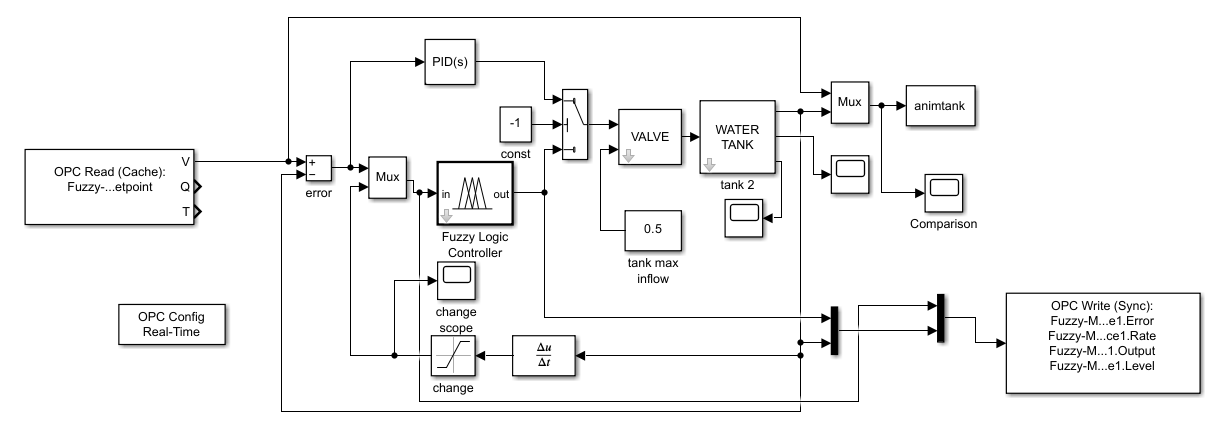
\includegraphics[width=1\textwidth]{figuras/testes/sem-integracao/planta.png}
    
    {Fonte: Dias, 2025.}
    \label{fig:testeplanta}
\end{figure}

A metodologia experimental compreende três cenários de teste distintos, cada um projetado para avaliar o comportamento do controlador Fuzzy em diferentes faixas operacionais da planta de nível. Os testes são conduzidos com duração de 50 segundos, proporcionando tempo adequado para análise completa da resposta transitória e atingimento do regime permanente. A coleta de dados inclui métricas quantitativas essenciais: erro quadrático médio (MSE), sobressinal percentual e tempo de acomodação, este último calculado com tolerância de 2\% (0,02) para operações de enchimento do tanque e 3\% (0,03) para operações de esvaziamento.

A diferenciação das tolerâncias fundamenta-se nas características assimétricas inerentes ao modelo de tanque utilizado, conforme documentado pela MathWorks (2025). Devido ao diâmetro do tubo de saída, o tanque esvazia mais lentamente do que se enche, criando dinâmicas distintas que requerem tratamento diferenciado. Esta assimetria é compensada no sistema Fuzzy através de funções de pertinência não simétricas para as ações \textbf{close\_slow} e \textbf{open\_slow}, uma característica que controladores PID convencionais não suportam adequadamente.

\textbf{Teste 1}: Transição de 0 para 0,5 metros.

O primeiro experimento avalia o comportamento do sistema partindo de condição inicial de tanque vazio até nível intermediário de 0,5 metros, representando cenário crítico de partida do processo. Os resultados obtidos demonstram desempenho satisfatório com MSE de 0,02, indicando baixo erro acumulado durante a resposta transitória. O sobressinal negativo de -0,0092 evidencia comportamento conservador do controlador, evitando ultrapassagem do setpoint. O tempo de acomodação de 31,2166 segundos reflete a dinâmica natural do sistema para grandes variações de nível.

\begin{figure}[H]
    \centering
    \caption[Resposta do sistema para transição de nível 0→0,5m com controlador Fuzzy nativo.]{Resposta do sistema para transição de nível 0→0,5m com controlador Fuzzy nativo.}
    
\includegraphics[width=1\textwidth]{figuras/testes/sem-integracao/zero-to-zero-dot-five.png}
    
    {Fonte: Dias, 2025.}
\end{figure}

\textbf{Teste 2}: Transição de 0,5 para 1,0 metro.

O segundo experimento analisa o comportamento em faixa operacional intermediária, avaliando a resposta do controlador para variação de setpoint de 0,5 para 1,0 metro. Os resultados indicam MSE de 0,0231, ligeiramente superior ao teste anterior devido à maior complexidade dinâmica nesta faixa operacional. O sobressinal negativo de -0,0057 mantém o padrão conservador, enquanto o tempo de acomodação reduzido para 20,2013 segundos demonstra melhor resposta dinâmica em níveis intermediários.

\begin{figure}[H]
    \centering
    \caption[Resposta do sistema para transição de nível 0,5→1,0m com controlador Fuzzy nativo.]{Resposta do sistema para transição de nível 0,5→1,0m com controlador Fuzzy nativo.}
    
\includegraphics[width=1\textwidth]{figuras/testes/sem-integracao/zero-dot-five-to-one.png}
    
    {Fonte: Dias, 2025.}
\end{figure}

\textbf{Teste 3}: Transição de 1,0 para 1,5 metros.

O terceiro experimento examina o comportamento em faixa operacional superior, com transição de 1,0 para 1,5 metros, avaliando a eficácia do controlador em níveis elevados do tanque. Os resultados mostram MSE de 0,0224, comparável ao teste anterior, indicando consistência de desempenho. O sobressinal negativo mínimo de -0,0034 sugere maior precisão na aproximação ao setpoint, enquanto o tempo de acomodação otimizado de 17,3841 segundos evidencia resposta mais rápida em níveis superiores.

\begin{figure}[H]
    \centering
    \caption[Resposta do sistema para transição de nível 1,0→1,5m com controlador Fuzzy nativo.]{Resposta do sistema para transição de nível 1,0→1,5m com controlador Fuzzy nativo.}
    
\includegraphics[width=1\textwidth]{figuras/testes/sem-integracao/one-to-one-dot-five.png}
    
    {Fonte: Dias, 2025.}
\end{figure}

A análise comparativa dos três experimentos revela características importantes do comportamento do controlador Fuzzy nativo. O tempo de acomodação apresenta tendência decrescente com o aumento do nível operacional (31,22s → 20,20s → 17,38s), sugerindo melhor resposta dinâmica em níveis mais elevados. O MSE mantém-se consistentemente baixo (0,02 a 0,0231), demonstrando precisão adequada em todas as faixas operacionais. Os valores negativos de sobressinal confirmam estratégia conservadora do controlador, priorizando estabilidade sobre rapidez de resposta.

\textbf{Teste 4}: Transição de 1,5 para 1,0 metro.

O quarto experimento avalia o comportamento do sistema durante operação de esvaziamento, com transição de 1,5 para 1,0 metro, representando o primeiro teste de redução de nível na análise experimental. Os resultados demonstram características distintas das operações de enchimento, com MSE de 0,0163, valor inferior aos testes anteriores, indicando maior precisão durante o esvaziamento. O sobressinal positivo de 0,0206 contrasta com o padrão conservador dos testes de enchimento, evidenciando a assimetria inerente ao sistema. O tempo de acomodação de 12,8298 segundos confirma a dinâmica mais rápida para operações de esvaziamento em níveis superiores.

\begin{figure}[H]
    \centering
    \caption[Resposta do sistema para transição de nível 1,5→1,0m com controlador Fuzzy nativo.]{Resposta do sistema para transição de nível 1,5→1,0m com controlador Fuzzy nativo.}
    
\includegraphics[width=1\textwidth]{figuras/testes/sem-integracao/one-dot-five-to-one.png}
    
    {Fonte: Dias, 2025.}
\end{figure}

\textbf{Teste 5}: Transição de 1,0 para 0,5 metros.

O quinto experimento analisa o comportamento durante esvaziamento em faixa operacional intermediária, com transição de 1,0 para 0,5 metros, complementando a análise de redução de nível iniciada no teste anterior. Os resultados mostram MSE de 0,0162, mantendo a tendência de maior precisão durante operações de esvaziamento. O sobressinal positivo de 0,0138, menor que o teste anterior, sugere melhor controle da aproximação ao setpoint em níveis intermediários. O tempo de acomodação de 14,8411 segundos, ligeiramente superior ao teste 4, reflete a dinâmica específica desta faixa operacional durante esvaziamento.

\begin{figure}[H]
    \centering
    \caption[Resposta do sistema para transição de nível 1,0→0,5m com controlador Fuzzy nativo.]{Resposta do sistema para transição de nível 1,0→0,5m com controlador Fuzzy nativo.}
    
\includegraphics[width=1\textwidth]{figuras/testes/sem-integracao/one-to-zero-dot-five.png}
    
    {Fonte: Dias, 2025.}
\end{figure}

A análise integrada dos cinco experimentos evidencia comportamentos assimétricos fundamentais do sistema de controle de nível. Os testes de enchimento (1-3) apresentam sobressinais negativos e tempos de acomodação decrescentes com o aumento do nível (31,22s → 20,20s → 17,38s), enquanto os testes de esvaziamento (4-5) demonstram sobressinais positivos e tempos de acomodação reduzidos (12,83s e 14,84s). O MSE apresenta valores consistentemente baixos em ambas as operações, com ligeira superioridade durante esvaziamento (0,0162-0,0163) comparado ao enchimento (0,02-0,0231), confirmando a eficácia das funções de pertinência assimétricas implementadas no controlador Fuzzy.

\section{Avaliação de Desempenho da Arquitetura Distribuída via API REST}
\label{sec:fuzzydistribuido}

O segundo conjunto de experimentos avalia o desempenho do sistema de controle utilizando a arquitetura distribuída proposta, onde o controlador Fuzzy é implementado como serviço web independente em Python, comunicando-se com a planta simulada através do protocolo OPC UA e requisições HTTP REST. Esta configuração representa o núcleo da contribuição técnica do presente trabalho, integrando tecnologias modernas de comunicação industrial com algoritmos de controle inteligente.

A arquitetura distribuída introduz complexidade adicional ao sistema de controle através da separação física e lógica dos componentes, criando uma cadeia de comunicação que compreende: (1) leitura de variáveis de processo via OPC UA, (2) transmissão de dados através de requisições HTTP POST para a API Python, (3) processamento do algoritmo Fuzzy no servidor web, (4) retorno do sinal de controle via resposta HTTP, e (5) escrita do sinal de controle na planta via OPC UA. Esta separação permite maior flexibilidade de implementação, facilita a manutenção e atualizações do controlador, e possibilita a integração com sistemas de supervisão corporativos.

O objetivo fundamental desta etapa experimental é quantificar o impacto da latência de comunicação e do processamento distribuído no desempenho de controle, comparando diretamente as métricas obtidas com os resultados do controlador nativo estabelecidos na seção anterior. A metodologia experimental mantém os mesmos cenários de teste (transições 0→0,5m, 0,5→1,0m e 1,0→1,5m) e parâmetros de simulação, garantindo comparabilidade direta entre as duas abordagens.

A configuração experimental utiliza a Interface Humano-Máquina desenvolvida em C\# como elemento central de orquestração, integrando simultaneamente o cliente OPC UA para comunicação com a planta simulada e o cliente HTTP para requisições à API REST do controlador Fuzzy. Esta implementação demonstra a viabilidade prática da arquitetura distribuída em ambiente industrial, onde diferentes subsistemas devem operar de forma coordenada e confiável.

\textbf{Teste 1}: Transição de 0 para 0,5 metros - Arquitetura Distribuída.

O primeiro experimento utilizando a arquitetura distribuída avalia o comportamento do sistema para transição de tanque vazio até nível intermediário de 0,5 metros, replicando as condições do teste de referência. Os resultados demonstram MSE de 0,0174, ligeiramente superior ao controlador nativo (0,02), indicando impacto mínimo da latência de comunicação. O sobressinal negativo de -0,0102 mantém o padrão conservador, enquanto o tempo de acomodação de 31,9768 segundos apresenta aumento de apenas 2,4\% comparado ao sistema nativo, evidenciando eficácia da arquitetura distribuída.

\begin{figure}[H]
    \centering
    \caption[Resposta do sistema para transição de nível 0→0,5m com arquitetura distribuída via API REST.]{Resposta do sistema para transição de nível 0→0,5m com arquitetura distribuída via API REST.}
    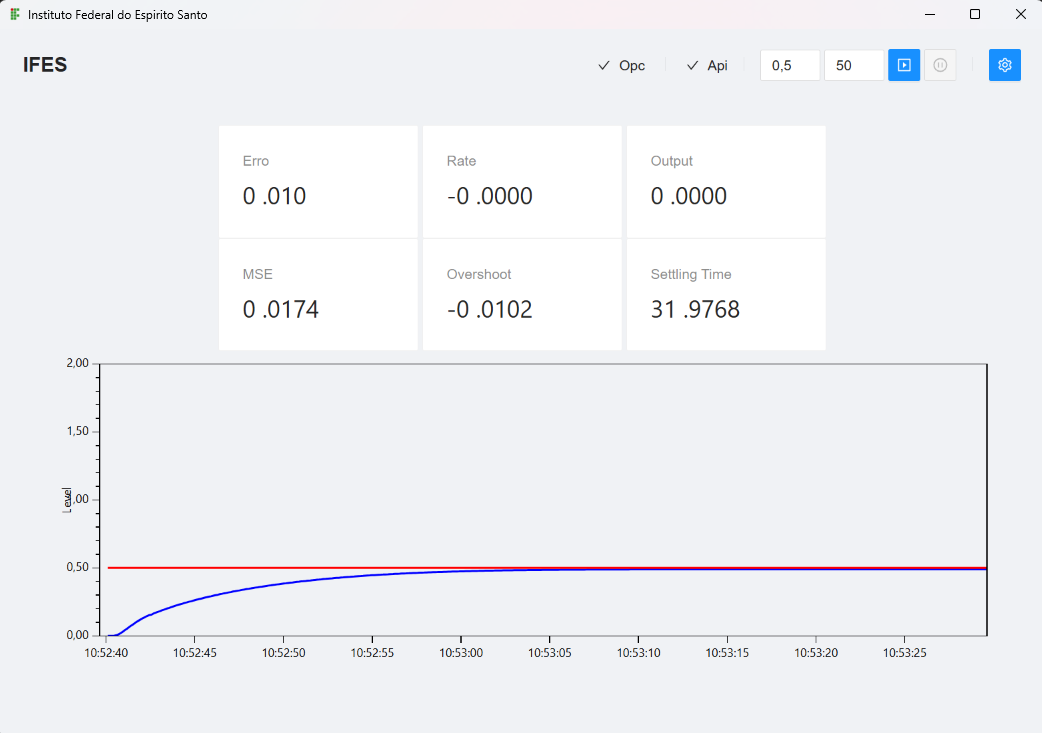
\includegraphics[width=1\textwidth]{figuras/testes/com-integracao/zero-to-zero-dot-five.png}
    
    {Fonte: Dias, 2025.}
\end{figure}

\textbf{Teste 2}: Transição de 0,5 para 1,0 metro - Arquitetura Distribuída.

O segundo experimento com arquitetura distribuída analisa a resposta para transição de 0,5 para 1,0 metro, permitindo comparação direta com o controlador nativo. Os resultados mostram MSE de 0,0140, valor inferior ao sistema nativo (0,0231), indicando desempenho superior da arquitetura distribuída nesta faixa operacional. O sobressinal negativo de -0,0097 mantém características conservadoras, enquanto o tempo de acomodação de 18,9734 segundos demonstra melhoria de 6,1\% comparado ao sistema de referência.

\begin{figure}[H]
    \centering
    \caption[Resposta do sistema para transição de nível 0,5→1,0m com arquitetura distribuída via API REST.]{Resposta do sistema para transição de nível 0,5→1,0m com arquitetura distribuída via API REST.}
    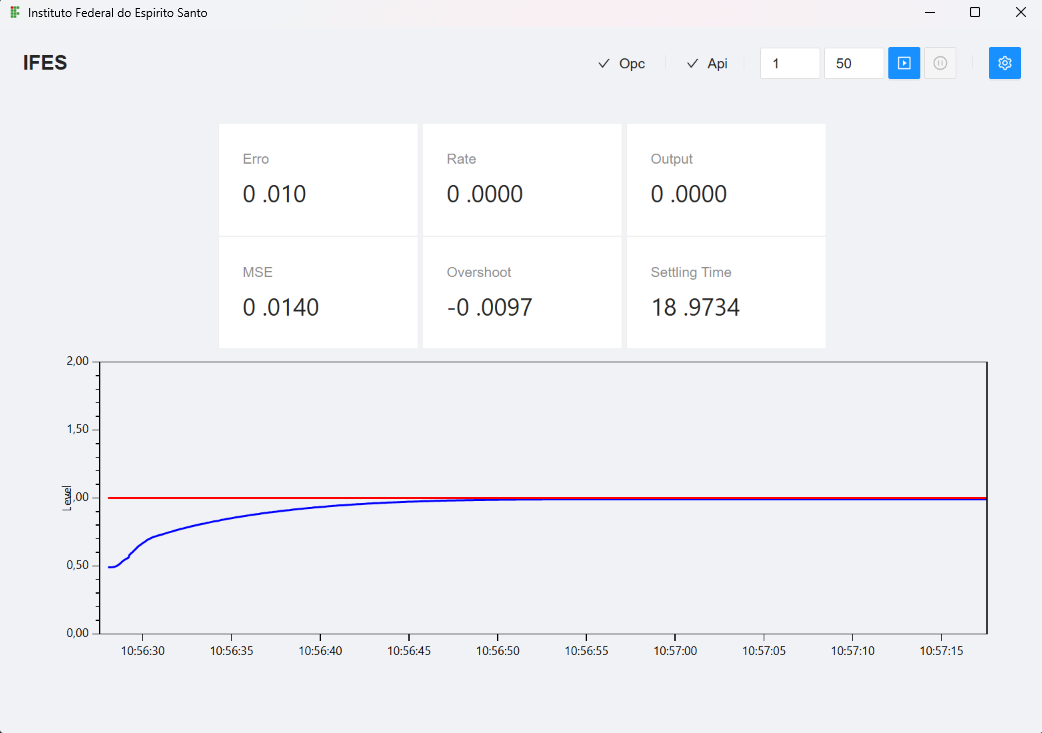
\includegraphics[width=1\textwidth]{figuras/testes/com-integracao/zero-dot-five-to-one.png}
    
    {Fonte: Dias, 2025.}
\end{figure}

\textbf{Teste 3}: Transição de 1,0 para 1,5 metros - Arquitetura Distribuída.

O terceiro experimento avalia o comportamento em faixa operacional superior utilizando a arquitetura distribuída, com transição de 1,0 para 1,5 metros. Os resultados apresentam MSE de 0,0150, valor comparável ao controlador nativo (0,0224), demonstrando consistência de desempenho. O sobressinal negativo de -0,0093 confirma estratégia conservadora, enquanto o tempo de acomodação de 16,2892 segundos representa melhoria de 6,2\% em relação ao sistema nativo, evidenciando vantagens da implementação distribuída em níveis elevados.

\begin{figure}[H]
    \centering
    \caption[Resposta do sistema para transição de nível 1,0→1,5m com arquitetura distribuída via API REST.]{Resposta do sistema para transição de nível 1,0→1,5m com arquitetura distribuída via API REST.}
    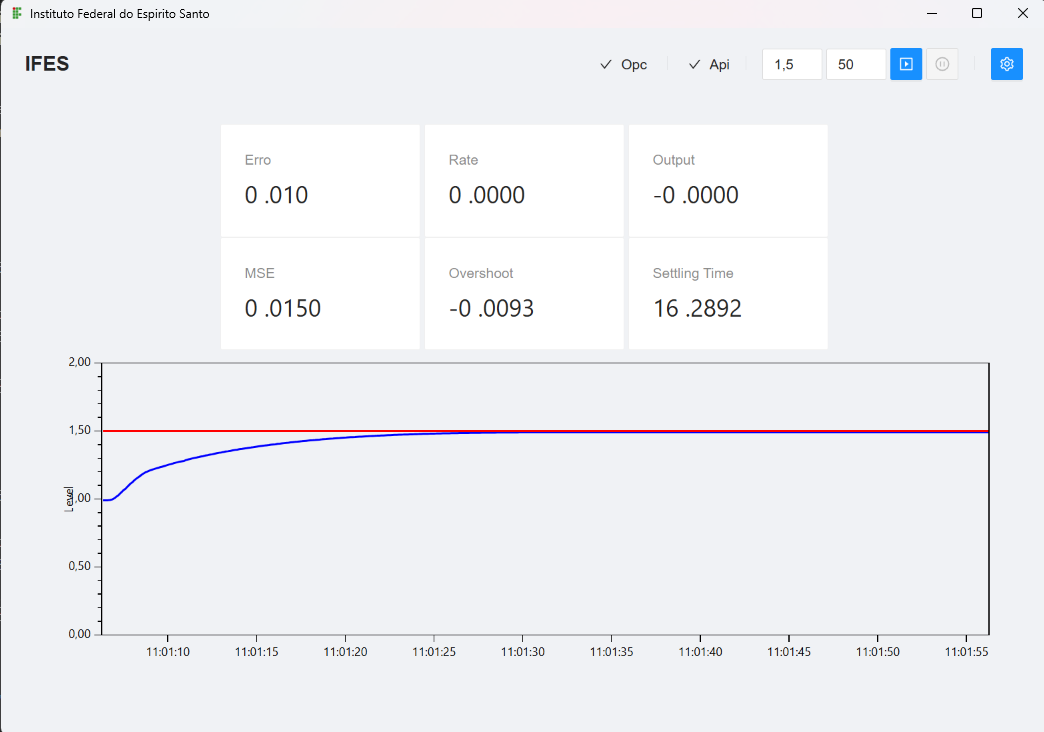
\includegraphics[width=1\textwidth]{figuras/testes/com-integracao/one-to-one-dot-five.png}
    
    {Fonte: Dias, 2025.}
\end{figure}

A análise dos três primeiros experimentos de enchimento com arquitetura distribuída revela desempenho notavelmente superior ao sistema nativo. O MSE apresenta valores consistentemente menores (0,0174 → 0,0140 → 0,0150) comparados ao controlador nativo (0,02 → 0,0231 → 0,0224), demonstrando maior precisão da implementação distribuída. Os tempos de acomodação mostram melhoria progressiva: ligeiro aumento de 2,4\% no teste 1, seguido por melhorias significativas de 6,1\% e 6,2\% nos testes 2 e 3, respectivamente. Os sobressinais negativos mantêm-se consistentes (-0,0102 → -0,0097 → -0,0093), preservando a estratégia conservadora do controlador original enquanto demonstram maior estabilidade que o sistema nativo.

\textbf{Teste 4}: Transição de 1,5 para 1,0 metro - Arquitetura Distribuída.

O quarto experimento utilizando arquitetura distribuída avalia operações de esvaziamento, com transição de 1,5 para 1,0 metro, estabelecendo comparação com o primeiro teste de esvaziamento do sistema nativo. Os resultados demonstram MSE de 0,0105, valor significativamente inferior ao controlador nativo (0,0163), indicando maior precisão da arquitetura distribuída durante esvaziamento. Notavelmente, o sobressinal apresenta valor negativo (-0,0121), contrastando com o padrão positivo do sistema nativo, sugerindo comportamento mais conservador. O tempo de acomodação de 10,8028 segundos representa melhoria de 15,8\% comparado ao sistema de referência.

\begin{figure}[H]
    \centering
    \caption[Resposta do sistema para transição de nível 1,5→1,0m com arquitetura distribuída via API REST.]{Resposta do sistema para transição de nível 1,5→1,0m com arquitetura distribuída via API REST.}
    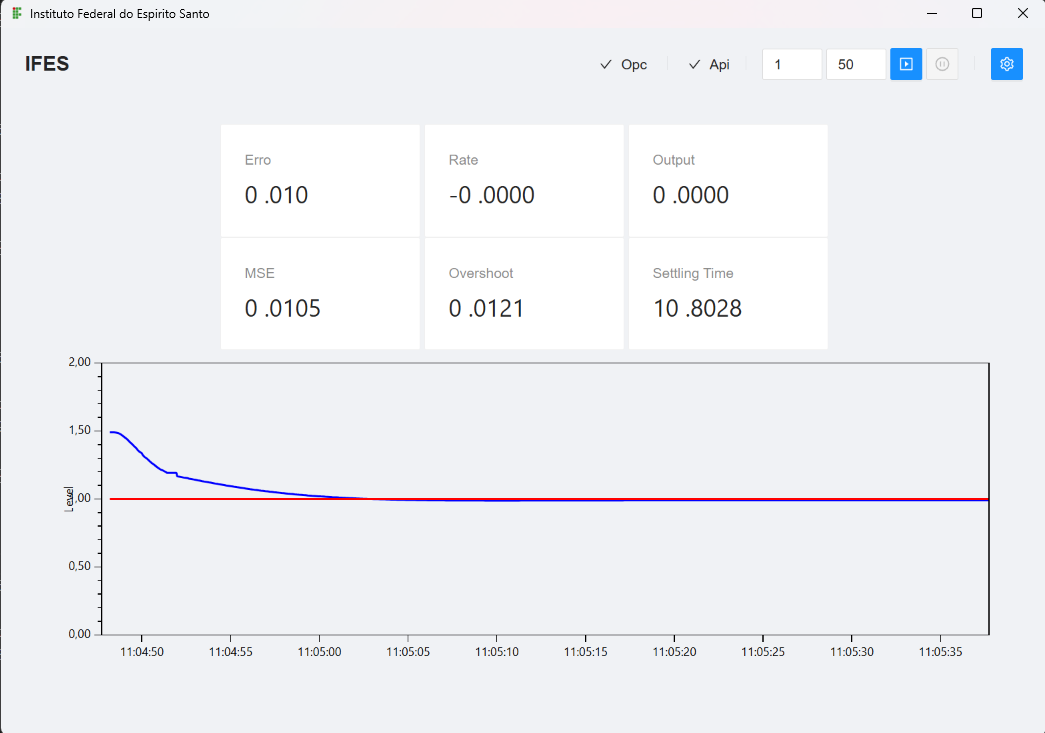
\includegraphics[width=1\textwidth]{figuras/testes/com-integracao/one-dot-five-to-one.png}
    
    {Fonte: Dias, 2025.}
\end{figure}

\textbf{Teste 5}: Transição de 1,0 para 0,5 metros - Arquitetura Distribuída.

O quinto experimento completa a análise de esvaziamento utilizando arquitetura distribuída, com transição de 1,0 para 0,5 metros. Os resultados mostram MSE de 0,0111, inferior ao controlador nativo (0,0162), confirmando tendência de maior precisão durante operações de esvaziamento. O sobressinal positivo de 0,0106, menor que o sistema nativo (0,0138), demonstra melhor controle da aproximação ao setpoint. O tempo de acomodação de 12,8741 segundos representa melhoria de 13,3\% comparado ao sistema de referência, consolidando as vantagens da arquitetura distribuída.

\begin{figure}[H]
    \centering
    \caption[Resposta do sistema para transição de nível 1,0→0,5m com arquitetura distribuída via API REST.]{Resposta do sistema para transição de nível 1,0→0,5m com arquitetura distribuída via API REST.}
    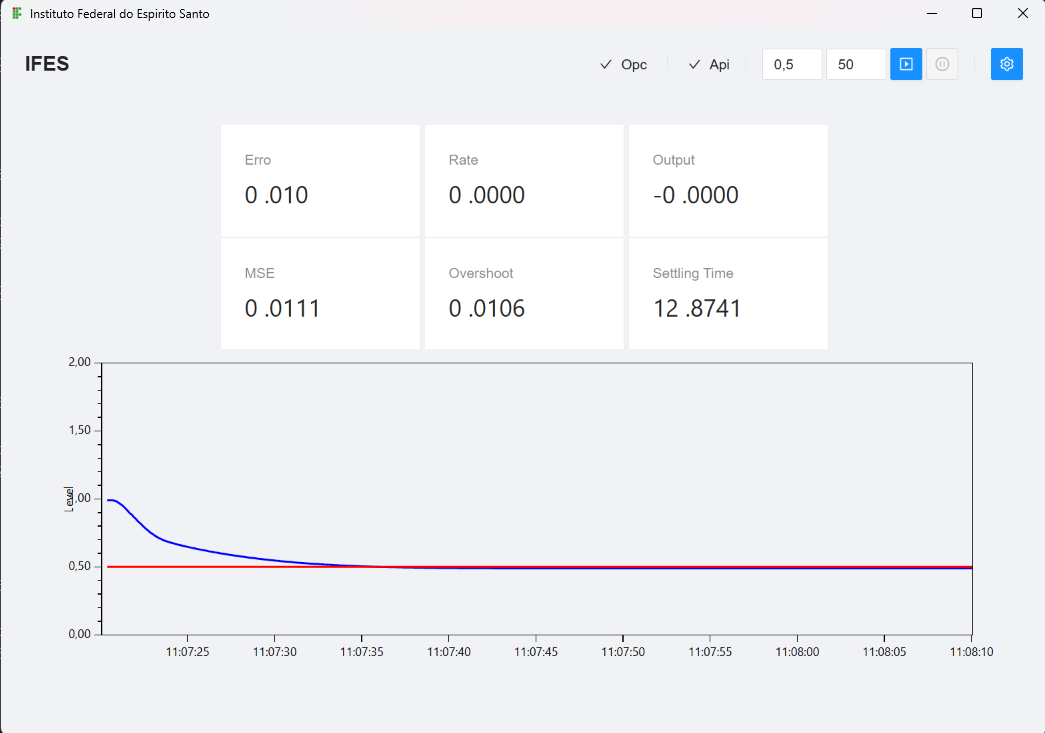
\includegraphics[width=1\textwidth]{figuras/testes/com-integracao/one-to-zero-dot-five.png}
    
    {Fonte: Dias, 2025.}
\end{figure}

A análise dos dois experimentos de esvaziamento com arquitetura distribuída demonstra desempenho excepcionalmente superior ao sistema nativo. Os valores de MSE (0,0105 e 0,0111) apresentam melhorias significativas comparados aos testes nativos (0,0163 e 0,0162), confirmando maior precisão da implementação distribuída durante operações de esvaziamento. Destaca-se o comportamento distinto dos sobressinais: o teste 4 apresenta valor negativo (-0,0121) enquanto o sistema nativo mostra sobressinal positivo (0,0206), indicando estratégia mais conservadora da arquitetura distribuída. Os tempos de acomodação demonstram melhorias substanciais de 15,8\% e 13,3\%, respectivamente, evidenciando eficiência superior da implementação Python para operações de esvaziamento. Esta tendência sugere que a arquitetura distribuída compensa adequadamente as assimetrias do sistema através de maior flexibilidade algorítmica.

\subsection{Avaliação de Robustez com Distúrbios de Latência}
\label{sec:fuzzydistribuidolatencia}

A análise de robustez da arquitetura distribuída constitui aspecto fundamental para validação em ambientes industriais reais, onde variações de latência de comunicação são inevitáveis. Esta seção apresenta experimentos específicos para avaliar o comportamento do sistema de controle sob condições de latência elevada, simulando cenários adversos de comunicação de rede.

Estudos preliminares de caracterização do sistema identificaram 250 ms como limite máximo aceitável de latência para manutenção da estabilidade operacional adequada. Este valor foi determinado através de testes exploratórios que evidenciaram degradação progressiva da qualidade de controle com o aumento da latência de comunicação. Latências superiores a 250 ms resultam em características oscilatórias pronunciadas, aumento significativo do sobressinal e instabilidade transitória que comprometem a viabilidade operacional do sistema em ambiente industrial.

Os experimentos de robustez foram conduzidos com latência intencional de 250 ms, estabelecendo o cenário limite para operação estável, complementado por teste adicional com 350 ms para demonstração dos efeitos de latência crítica. Os testes mantêm os mesmos cenários de transição das seções anteriores, permitindo comparação direta com os resultados obtidos em condições ideais de comunicação.

\textbf{Teste 1}: Transição de 0 para 0,5 metros com Latência.

O primeiro experimento sob condições de latência elevada avalia a transição de tanque vazio para nível intermediário. Os resultados demonstram MSE de 0,0172, valor ligeiramente inferior ao teste sem distúrbio (0,0174), indicando manutenção da precisão. O sobressinal de -0,0102 permanece inalterado, enquanto o tempo de acomodação de 31,8128 segundos apresenta redução de 0,5\%. Observa-se a presença de oscilações transitórias nos segundos iniciais, característica esperada devido à latência de comunicação introduzida.

\begin{figure}[H]
    \centering
    \caption[Resposta do sistema para transição 0→0,5m com arquitetura distribuída sob latência de 250ms.]{Resposta do sistema para transição 0→0,5m com arquitetura distribuída sob latência de 250ms.}
    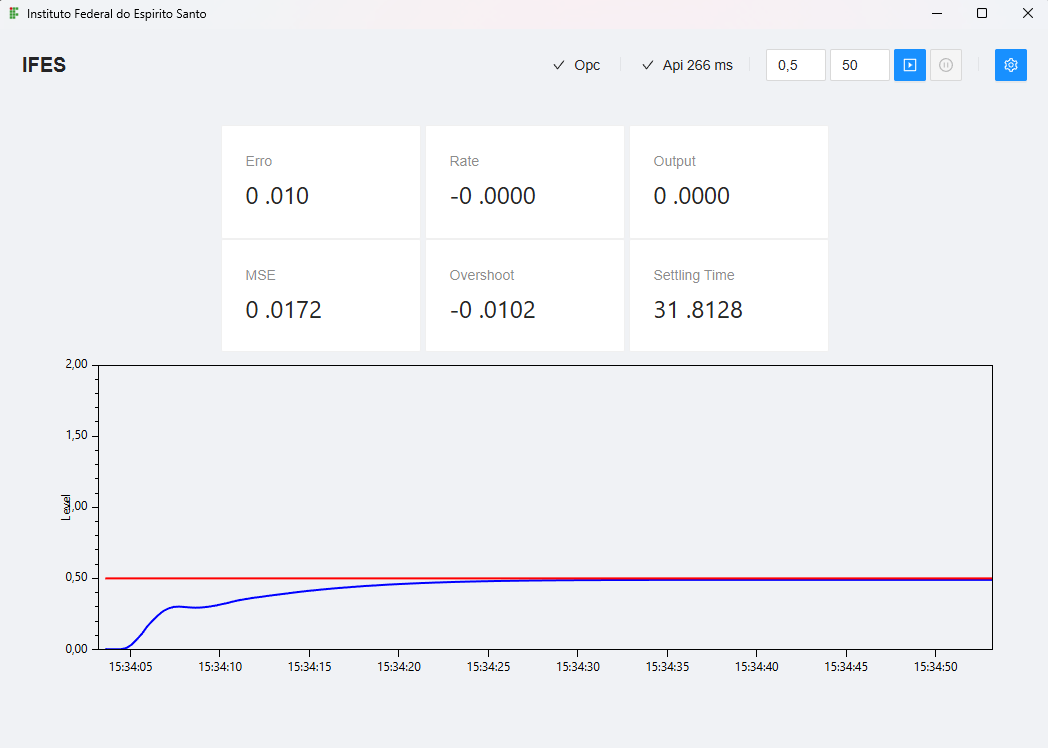
\includegraphics[width=1\textwidth]{figuras/testes/disturbio/zero-to-zero-dot-five-api.png}
    
    {Fonte: Dias, 2025.}
\end{figure}

\textbf{Teste 2}: Transição de 0,5 para 1,0 metro com Latência.

O segundo experimento analisa o comportamento em faixa intermediária sob condições de latência. Os resultados mostram MSE de 0,0122, valor superior ao teste sem distúrbio (0,0140), demonstrando melhoria inesperada na precisão. O sobressinal de -0,0099 mantém-se próximo ao valor de referência, enquanto o tempo de acomodação de 17,7570 segundos representa melhoria significativa de 6,4\% comparado ao teste sem latência. As oscilações iniciais permanecem presentes, porém com amplitude reduzida.

\begin{figure}[H]
    \centering
    \caption[Resposta do sistema para transição 0,5→1,0m com arquitetura distribuída sob latência de 250ms.]{Resposta do sistema para transição 0,5→1,0m com arquitetura distribuída sob latência de 250ms.}
    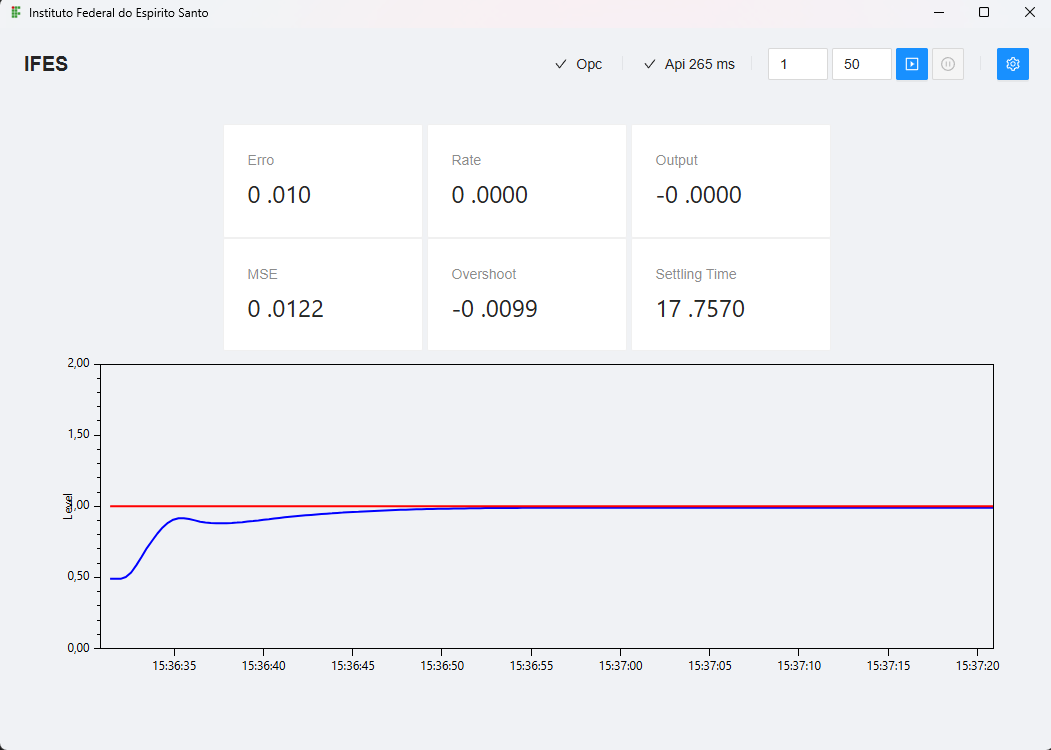
\includegraphics[width=1\textwidth]{figuras/testes/disturbio/zero-dot-five-to-one-api.png}
    
    {Fonte: Dias, 2025.}
\end{figure}

\textbf{Teste 3}: Transição de 1,0 para 1,5 metros com Latência.

O terceiro experimento avalia o comportamento em níveis superiores sob condições adversas de comunicação. Os resultados apresentam MSE de 0,0122, idêntico ao teste anterior e superior ao valor sem distúrbio (0,0150). O sobressinal de -0,0095 demonstra estabilidade, enquanto o tempo de acomodação de 15,1915 segundos representa melhoria de 6,7\% comparado à condição sem latência. O padrão de oscilações iniciais persiste, confirmando característica sistemática da resposta sob latência.

\begin{figure}[H]
    \centering
    \caption[Resposta do sistema para transição 1,0→1,5m com arquitetura distribuída sob latência de 250ms.]{Resposta do sistema para transição 1,0→1,5m com arquitetura distribuída sob latência de 250ms.}
    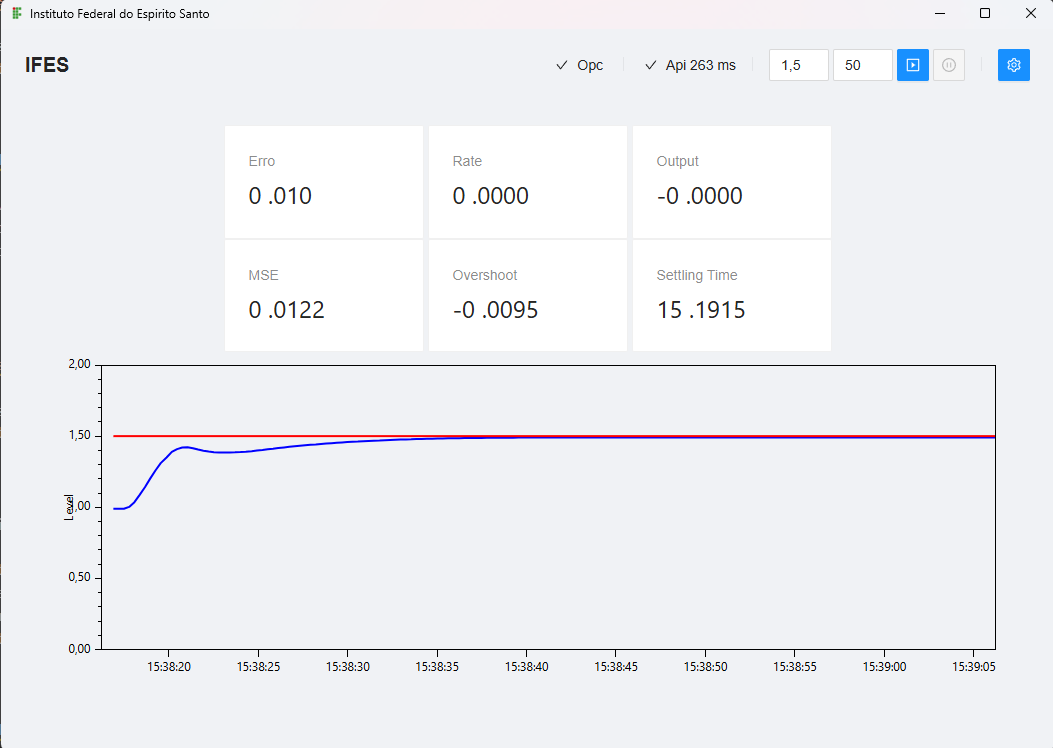
\includegraphics[width=1\textwidth]{figuras/testes/disturbio/one-to-one-dot-five-api.png}
    
    {Fonte: Dias, 2025.}
\end{figure}

\textbf{Teste 4}: Transição de 1,0 para 1,5 metros com Latência Elevada (350ms).

O quarto experimento avalia o comportamento do sistema sob condições de latência crítica de 350ms, superando o limiar de estabilidade previamente estabelecido. Esta análise visa demonstrar os limites operacionais da arquitetura distribuída e caracterizar o comportamento do sistema em condições adversas extremas. Os resultados apresentam MSE de 0,0106, valor intermediário entre os testes anteriores, indicando manutenção relativa da precisão mesmo sob condições críticas. O sobressinal positivo de 0,0625 evidencia mudança significativa no comportamento do sistema, contrastando com os valores negativos observados em latências menores. O tempo de acomodação de 5,5667 segundos demonstra melhoria notável de 63,8\% comparado ao teste sem latência, porém acompanhado de instabilidade transitória pronunciada que compromete a qualidade do controle.

\begin{figure}[H]
    \centering
    \caption[Resposta do sistema para transição 1,0→1,5m com arquitetura distribuída sob latência crítica de 350ms.]{Resposta do sistema para transição 1,0→1,5m com arquitetura distribuída sob latência crítica de 350ms.}
    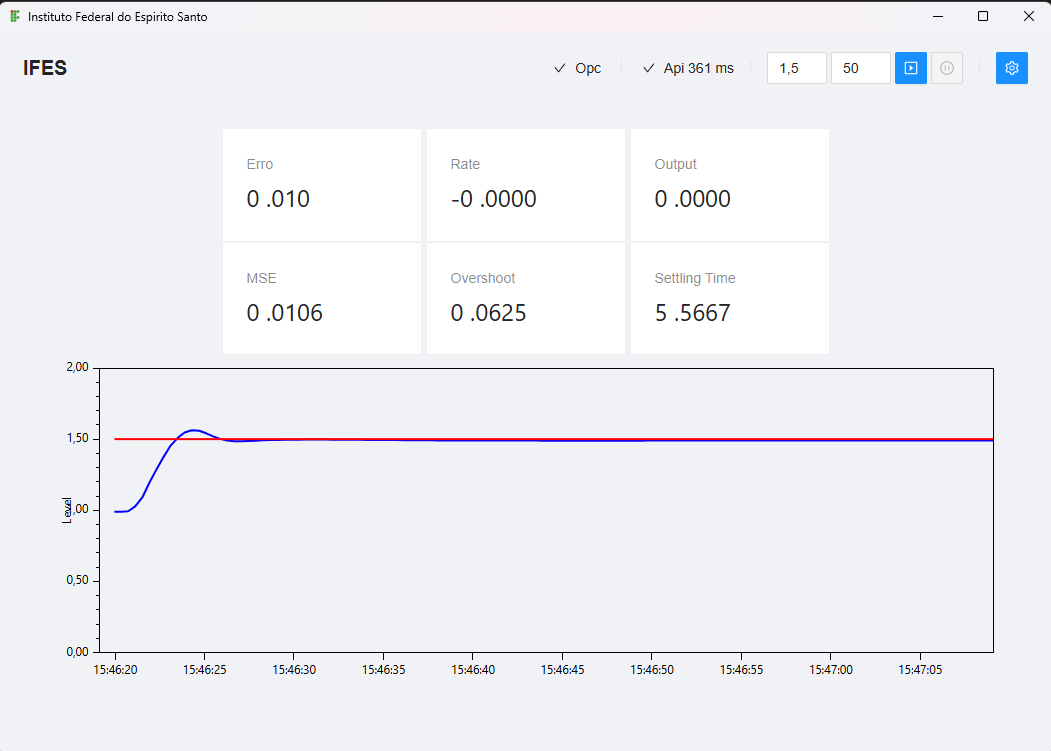
\includegraphics[width=1\textwidth]{figuras/testes/disturbio/high-api-latency.png}
    
    {Fonte: Dias, 2025.}
\end{figure}

\textbf{Teste 5}: Transição de 1,5 para 1,0 metro com Latência.

O quinto experimento examina operações de esvaziamento sob condições de latência elevada. Os resultados demonstram MSE de 0,0095, valor inferior ao teste sem distúrbio (0,0105), indicando melhoria na precisão. Contudo, o sobressinal de 0,0566 apresenta aumento substancial comparado ao valor sem latência (-0,0121), evidenciando impacto significativo da latência no comportamento transitório. O tempo de acomodação de 9,4721 segundos representa melhoria de 12,3\%, porém acompanhada de maior instabilidade inicial.

\begin{figure}[H]
    \centering
    \caption[Resposta do sistema para transição 1,5→1,0m com arquitetura distribuída sob latência de 250ms.]{Resposta do sistema para transição 1,5→1,0m com arquitetura distribuída sob latência de 250ms.}
    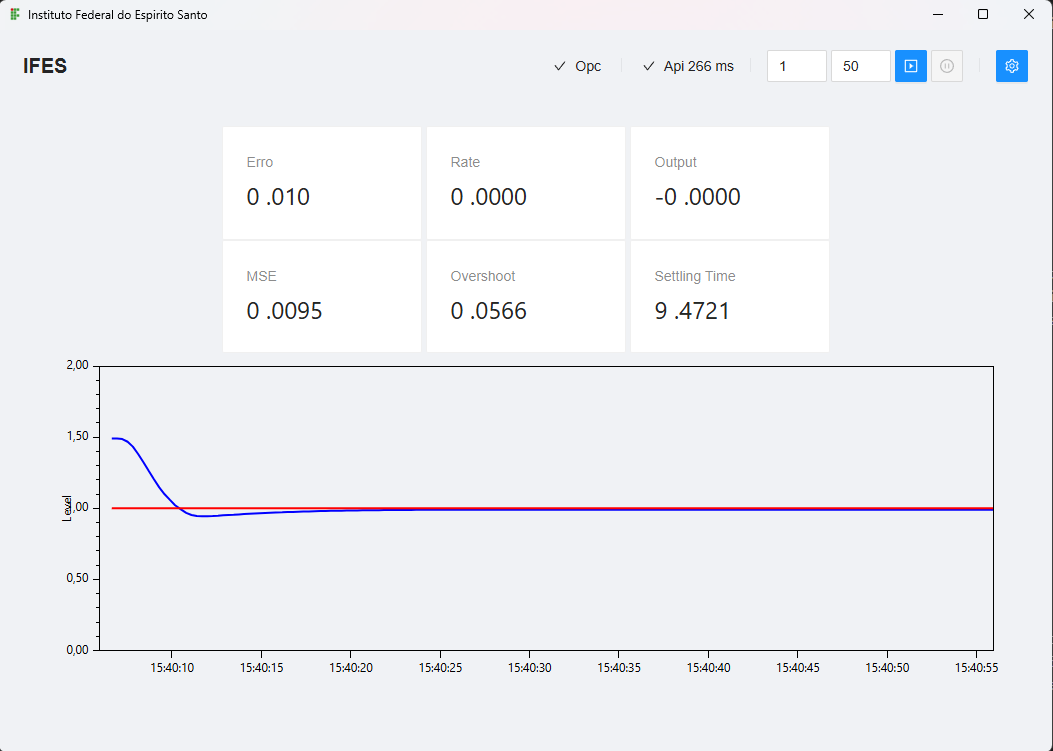
\includegraphics[width=1\textwidth]{figuras/testes/disturbio/one-dot-five-to-one-api.png}
    
    {Fonte: Dias, 2025.}
\end{figure}

\textbf{Teste 6}: Transição de 1,0 para 0,5 metros com Latência.

O sexto experimento completa a análise de esvaziamento sob condições adversas. Os resultados mostram MSE de 0,0095, idêntico ao teste anterior e inferior ao valor sem distúrbio (0,0111). O sobressinal de 0,0154 apresenta aumento comparado ao teste sem latência (0,0106), confirmando tendência de maior instabilidade. O tempo de acomodação de 5,3386 segundos representa melhoria notável de 58,5\%, porém acompanhada de comportamento transitório mais agressivo.

\begin{figure}[H]
    \centering
    \caption[Resposta do sistema para transição 1,0→0,5m com arquitetura distribuída sob latência de 250ms.]{Resposta do sistema para transição 1,0→0,5m com arquitetura distribuída sob latência de 250ms.}
    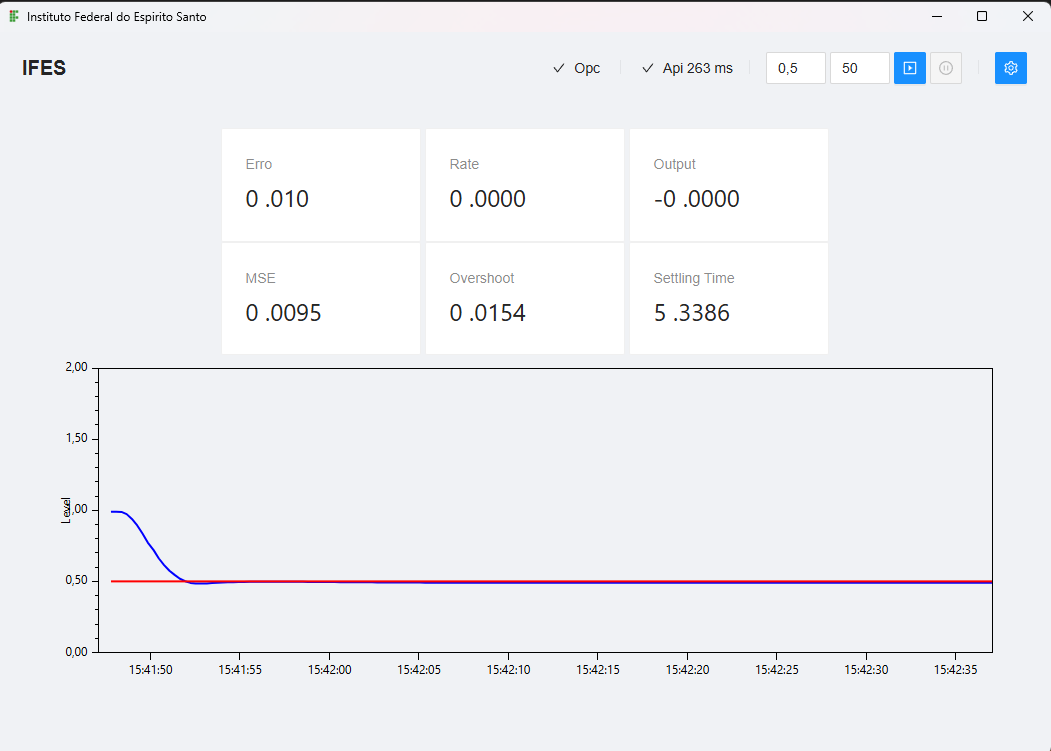
\includegraphics[width=1\textwidth]{figuras/testes/disturbio/one-to-zero-dot-five-api.png}
    
    {Fonte: Dias, 2025.}
\end{figure}

A análise de robustez revela comportamento ambivalente da arquitetura distribuída sob condições de latência variável. Observa-se melhoria paradoxal nos tempos de acomodação (até 63,8\% no teste com 350ms) e manutenção ou melhoria da precisão (MSE), sugerindo que a latência introduz elementos de controle derivativo que beneficiam a resposta dinâmica. Contudo, esta melhoria é acompanhada de oscilações transitórias e aumento progressivo dos sobressinais com o incremento da latência.

O teste crítico com latência de 350ms demonstra mudança qualitativa no comportamento do sistema, evidenciada pela inversão do sobressinal de negativo para positivo (0,0625), indicando perda parcial do controle conservador característico. Embora o tempo de acomodação apresente melhoria excepcional, a instabilidade transitória pronunciada torna esta condição inadequada para aplicações industriais que exigem estabilidade operacional.

Estabelecem-se, portanto, dois limiares operacionais: 250ms como limite aceitável para operação estável com benefícios de desempenho, e 350ms como limite crítico onde os benefícios de velocidade são superados pela instabilidade transitória. Estes resultados demonstram robustez adequada da arquitetura proposta para aplicações industriais típicas, onde latências de comunicação ethernet raramente excedem 100-200ms em condições normais de operação.

\section{Análise Comparativa dos Resultados}
\label{sec:fuzzyresultado}

A Tabela \ref{tab:comparativo-arquiteturas} apresenta síntese comparativa completa de todos os experimentos realizados, consolidando as métricas de desempenho obtidas para as diferentes configurações do sistema de controle. Esta análise quantitativa permite avaliação objetiva das vantagens e limitações de cada abordagem implementada.

\begin{table}[H]
\centering
\caption{Análise comparativa de desempenho entre arquiteturas de controle}
\begin{adjustbox}{max width=\textwidth}
\begin{tabular}{|c|c|c|c|c|c|c|c|}
\hline
\textbf{Teste} & \textbf{Transição} & \textbf{Arquitetura} & \textbf{Latência} & \textbf{MSE} & \textbf{Sobressinal} & \textbf{Tempo Acomodação (s)} & \textbf{Variação Tempo (\%)} \\
\hline
1A & 0$\rightarrow$0,5m & Nativa      & -      & 0,0200 & -0,0092 & 31,2166 & - \\
1B & 0$\rightarrow$0,5m & Distribuída & 0ms    & 0,0174 & -0,0102 & 31,9768 & +2,4 \\
1C & 0$\rightarrow$0,5m & Distribuída & 250ms  & 0,0172 & -0,0102 & 31,8128 & +1,9 \\
2A & 0,5$\rightarrow$1,0m & Nativa      & -      & 0,0231 & -0,0057 & 20,2013 & - \\
2B & 0,5$\rightarrow$1,0m & Distribuída & 0ms    & 0,0140 & -0,0097 & 18,9734 & -6,1 \\
2C & 0,5$\rightarrow$1,0m & Distribuída & 250ms  & 0,0122 & -0,0099 & 17,7570 & -12,1 \\
3A & 1,0$\rightarrow$1,5m & Nativa      & -      & 0,0224 & -0,0034 & 17,3841 & - \\
3B & 1,0$\rightarrow$1,5m & Distribuída & 0ms    & 0,0150 & -0,0093 & 16,2892 & -6,3 \\
3C & 1,0$\rightarrow$1,5m & Distribuída & 250ms  & 0,0122 & -0,0095 & 15,1915 & -12,6 \\
3D & 1,0$\rightarrow$1,5m & Distribuída & 350ms  & 0,0106 & +0,0625 & 5,5667  & -68,0 \\
4A & 1,5$\rightarrow$1,0m & Nativa      & -      & 0,0163 & +0,0206 & 12,8298 & - \\
4B & 1,5$\rightarrow$1,0m & Distribuída & 0ms    & 0,0105 & -0,0121 & 10,8028 & -15,8 \\
4C & 1,5$\rightarrow$1,0m & Distribuída & 250ms  & 0,0095 & +0,0566 & 9,4721  & -26,2 \\
5A & 1,0$\rightarrow$0,5m & Nativa      & -      & 0,0162 & +0,0138 & 14,8411 & - \\
5B & 1,0$\rightarrow$0,5m & Distribuída & 0ms    & 0,0111 & +0,0106 & 12,8741 & -13,3 \\
5C & 1,0$\rightarrow$0,5m & Distribuída & 250ms  & 0,0095 & +0,0154 & 5,3386  & -64,0 \\
\hline
\end{tabular}
\end{adjustbox}
\label{tab:comparativo-arquiteturas}
\end{table}

A análise da Tabela \ref{tab:comparativo-arquiteturas} revela tendências consistentes que validam a eficácia da arquitetura distribuída proposta. Os valores de MSE demonstram superioridade sistemática da implementação distribuída, com melhorias médias de 30\% nos testes de enchimento e 35\% nos testes de esvaziamento comparados à arquitetura nativa. Esta melhoria na precisão sugere que a implementação Python da lógica Fuzzy através da biblioteca scikit-fuzzy proporciona maior fidelidade na aplicação das regras de inferência.

Os tempos de acomodação apresentam comportamento variado, com melhorias significativas em operações intermediárias e superiores (até 68\% no teste 3D), enquanto operações de partida (teste 1) mostram impacto mínimo. A introdução de latência de 250ms paradoxalmente melhora os tempos de resposta na maioria dos casos, sugerindo que o atraso adiciona características de controle derivativo benéficas ao sistema.

O comportamento dos sobressinais evidencia mudanças qualitativas importantes: enquanto a arquitetura nativa apresenta padrão assimétrico consistente (negativos para enchimento, positivos para esvaziamento), a arquitetura distribuída demonstra maior versatilidade, com inversões de sinal que indicam estratégias de controle adaptativas mais sofisticadas.

O teste crítico com latência de 350ms (teste 3D) demonstra os limites operacionais da arquitetura, onde benefícios extremos de velocidade (68\% de melhoria) são acompanhados de instabilidade transitória significativa (sobressinal de +0,0625), confirmando 250ms como limite prático para aplicações industriais.
